\documentclass{mbe}
\usepackage{natbib}
\setlength{\bibsep}{0.0pt}

\begin{document}

\newcommand{\pranka}{PRANK\_A}
\newcommand{\prankc}{PRANK\_C}
\newcommand{\omg}{\bm{\omega}}
\newcommand{\tpr}{TPR$_{1\%}$}

\title{The effects of alignment error and alignment filtering on the sitewise detection of positive selection}

\author{{Gregory Jordan and Nick Goldman}\\
\affiliation{European Bioinformatics Institute, Wellcome Trust Genome Campus, Hinxton, Cambridgeshire, CB10 1SD, United Kingdom}}
\authorlist{Jordan and Goldman}
\shorttitle{Alignment eror and detecting sitewise positive selection}

\mbeabstract{% 

The effects of alignment error on many types of evolutionary inference
are not well understood. Alignment filters are commonly applied to try
to reduce error rates resulting from misalignment, but neither the
quantitative impact of misalignment nor the ability of filters to
minimize such error has been systematically studied. We performed
simulation experiments to quantify the level of false positive and
false negative for sitewise detection of positive selection due to
misalignment and the ability of alignment filters to minimize
alignment-induced error. We find that while misalignment causes few
false positives when analyzing mammalian-like datasets with an
effective aligner, analyses at vertebrate-like or greater divergences
with either a poor aligner or a small number of sequences results in
high false positive rates.

}

\keywords{Positive selection, multiple alignment, alignment filtering, likelihood.}

\email{greg@ebi.ac.uk}

\mbestyle

\section*{Introduction}

Large-scale comparative genomics has been widely employed to identify
shared and unique biological features between organisms of interest to
the biomedical sciences, with applications ranging from evolutionary
annotation transfer \citep{Bork1998Predicting} to phylogenetics
\citep{Murphy2007Using,Prasad2008Confirming} and population genetic
inference \citep{Hurst2009Genetics}. The decreasing cost of DNA
sequencing has triggered a striking increase in the number of model
and non-model organisms with planned genome sequencing projects,
suggesting that the range and scale of comparative genomics
applications will continue to expand
\citep{Green20072x,2007Identification}.

The study of protein evolutionary rates and selective pressures in
particular has flourished as a result of the growth in comparative
genomics datasets. Clusters of closely-related genome sequences across
a wide taxonomic range have led to a better understanding of which
aspects of molecular evolution are variable and which are constant
\citep{Wolf2009Nonlinear}, and an increased sampling of species should
continue to boost the power and accuracy of individual analyses within
a given clade. This is especially beneficial for the calculation of
spatially precise evolutionary estimates, as additional species
sampling has been shown to be an effective means of boosting the
accuracy and power of sitewise detection of positive selection and
evolutionary constraint
\citep{Anisimova2001Accuracy,Massingham2005Detecting}. Site-specific
evolutionary estimates have proved especially valuable when analyzed
in conjunction with other protein-based datasets such as protein
structural features \citep{Lin2007Proportion,Ramsey2011Relationship},
human population diversity \citep{2010Map}, and human disease
mutations \citep{Arbiza2006Selective}.

A major concern in the sitewise detection of protein positive
selection is that the effect of alignment error is not well
characterized. Intuitively, one might expect alignment error to result
mainly in an increased number of false positives, as the spurious
alignment of nonhomologous codons on average would result in a high
number of apparent non-synonymous substitutions and a low number of
synonymous substitutions (since a randomly chosen pair of codons are
more likely to be nonsynonymous than synonymous). However, false
negatives may also be introduced, either through over-alignment of
synonymous codons (increasing the synonymous substitution rate) or
non-alignment of homologous codons (causing reduced power due to less
evolutionary information). Since different aligners employ a variety
of algorithms, evolutionary models, and heuristic optimizations
\citep{Notredame2007Recent}, each program may be more or less prone to different
types of alignment error, causing potentially large variations in the
nature and magnitude of its impact on the detection of positive
selection.

The protein structure and the evolutionary divergence of a dataset may
also contribute to the effects of alignment error. Differently
structured protein regions show variable tolerance to biological
indels, with indels more common in extracellular and transmembrane
proteins than in highly folded enzymes and housekeeping genes
\citep{delaChaux2007DNA} . This suggests that well-folded protein
regions will experience fewer biological indels -- and will therefore
be less susceptible to alignment error -- than less structured
regions. Furthermore, the evolutionary divergence of a dataset affects
the power of sitewise inference and the prevalence of indels in
different ways. Because maximum-likelihood methods for detecting
positive selection require data in the form of observed substitution
events, they show little power at low divergence and their highest
power at intermediate to high divergence levels
\citep{Anisimova2001Accuracy}. On the other hand, the number of indels
in a dataset should increase monotonically with divergence. These two
trends suggest that the overall power will be low at both extremes of
divergence, with little inference power at low divergences (due to the
scarcity of data in the form of observed substitutions) and an
overwhelming amount of alignment error at high divergences (due to the
large number of indel events). It is important to note, however, that
the majority of genes in many biological clades of interest (such as
mammals, vertebrates, fruit flies, and yeast) fall within the middle
range of divergences where sitewise methods are at their most powerful
and where multiple alignment is a difficult---but not
hopeless---problem. As such, it is important to seek an understanding
of the impact of alignment error on overall error rates within this
important range of divergence levels.

A number of empirical analyses have established that errors in gene
sequencing, annotation and alignment can contribute to errors in
downstream evolutionary analyses such as phylogeny inference
\citep{Wong2008Alignment} et and estimates of positive selection
\citep{Schneider2009Estimates,Markova-Raina2011High} . Most recently,
Markova-Raina et al. \citeyearpar{Markova-Raina2011High} showed that
the detection of positively-selected sites and genes in Drosophila
genomes is highly sensitive to aligner choice, with PRANK's codon
model consistently producing alignments with the lowest amount of
positive selection. Still, according to the authors' manual inspection
of alignments, even positively-selected sites identified with PRANK
alignments contained a sizable proportion of apparent false positives.

A limitation to the analysis of error in empirical datasets is the
lack of a benchmark set of true alignments and positively-selected
sites. Markova-Raina et al. \citeyearpar{Markova-Raina2011High} used
the expected general effect of alignment error (an increase in false
positives due to misalignment of non-homologous codons) as a proxy by
which to compare different methods, allowing for the conclusion that
PRANK was the least error-prone aligner in their analysis. However,
the absolute number of false positives remained uncertain due to the
possible conflation of multiple sources of error: in addition to
alignment error, the authors noted that gene mis-annotation was
responsible for many apparent false positives, and there was also an
expected error rate from the likelihood inference method itself. This
limitation leaves important and interesting questions regarding the
nature of misalignment error and its quantitative impact on the
detection of positive selection left unanswered.

Controlled simulation experiments provide a natural framework for
investigating error rates in detail, allowing one to pinpoint the
source of errors in multi-step analyses such as alignment followed by
evolutionary inference. This approach has widely been employed in
assessing the robustness of phylogenetic inference methods to
misalignment
\citep{Dwivedi2009Phylogenetic,Ogden2006Multiple,Loytynoja2008PhylogenyAware}
but those results cannot be easily extrapolated to the analysis of
sitewise selective pressures. More recently, Fletcher and Yang
\citeyearpar{Fletcher2010Effect} performed a series of simulation
experiments investigating alignment error in the use of branch-site
models to detect positive selection in genes. Their results showed
that most aligners caused false positives by over-aligning codons, and
that datasets from mammalian and vertebrate gene families contain
enough evolutionary divergence to make errors resulting from
misalignment a legitimate concern.

Reflecting a widespread awareness of the problem of misalignment,
methods for identifying and removing uncertain or unreliable alignment
regions have been commonly used in phylogenetic and molecular
evolutionary analyses. The popular Gblocks applies a set of heuristic
criteria (including thresholds on the amount of conservation and
gappiness) to identify conserved blocks deemed suitable for
phylogenetic or evolutionary analysis \citep{Castresana2000Selection},
while aligners such as T-Coffee \citep{Notredame2000TCoffee} and PRANK
\citep{Loytynoja2005From} produce estimates of alignment confidence or
reliability. Most recently, alignment confidence scores based on the
robustness of alignments to guide tree perturbations
\citep{Penn2010Alignment} or the sampling of suboptimal alignments
\citep{Kim2011PSAR} have been proposed. Unfortunately, despite their
widespread use, the impact of the many available filtering methods on
phylogenetic and evolutionary analyses has not been well-studied. Even
for a single filtering program, Gblocks, results have been
contradictory: one simulation-based study found that it improved the
phylogenetic signal \citep{Talavera2007Improvement} while an empirical
study across a wide range of taxa found that Gblocks-filtered
alignments produced worse phylogenetic trees
\citep{Dessimoz2010Phylogenetic}. The effect of filtering alignments
on the detection of positive selection is largely unexplored, although
it has become accepted practice to apply published filtering methods
before testing for positive selection \citep{Studer2008Pervasive,Aguileta2009Rapidly}.

This paper aims to use a simulation framework to incorporate
misalignment and alignment filtering into estimates of the power and
accuracy of sitewise evolutionary estimates. Our approach is similar
to that of Anisimova and Yang \citeyearpar{Anisimova2002Accuracy} in
that we use simulated protein alignments to evaluate methods for
detecting sitewise positive selection, considering each site to be an
independent hypothesis test producing a positive or negative
result. Our experimental design also shares some features with
Fletcher and Yang's \citeyearpar{Fletcher2010Effect} investigation of
the performance of branch-site methods for detecting genewise positive
selection under alignment error. Like Fletcher and Yang
\citeyearpar{Fletcher2010Effect}, we simulate codon alignments with
indels and calculate inferred alignments using a small but diverse
sample of aligners. Unlike their study, however, we focus on sitewise
detection of positive selection occurring throughout a phylogeny (as
opposed to genewise detection of selection acting at specific
branches), we explore a wider range of plausible tree sizes, indel
rates and divergence levels, and we evaluate the effects of a number
of alignment filtering methods on the error rate and power of sitewise
analysis. Given the recent proliferation of completed and planned
vertebrate genomes, we pay special attention to choosing simulation
parameters and analysis methods similar to those commonly encountered
in the sitewise analysis of vertebrate gene families.

\section*{Methods}

\subsection*{Alignment Simulations}

Three rooted trees were used to guide the simulation of protein-coding
DNA alignments: the artificial 6-taxon tree used by Anisimova and Yang
\citeyearpar{Anisimova2001Accuracy} and Massingham and Goldman
\citeyearpar{Massingham2005Detecting} rooted at its midpoint, the
17-taxon vertebrate B-globin tree from Yang et
al. \citeyearpar{Yang2000CodonSubstitution}, and the 44-taxon
vertebrate tree used by the ENCODE project
\citep{2007Identification,Nikolaev2007Early}. Trees, shown with their
original branch lengths in Figure 1, were scaled to comparable
divergence levels by normalizing their root-to-tip mean path length
(MPL), defined as the root-to-tip branch length averaged across all
lineages in the tree. We simulated alignments with MPL divergence
between 0.2 and 2.0 synonymous substitutions per synonymous site,
spanning the range of evolutionary divergences observed in several
clades of organisms with fully-sequenced genomes (Table ST1).

\begin{figure}[h]
\begin{center}
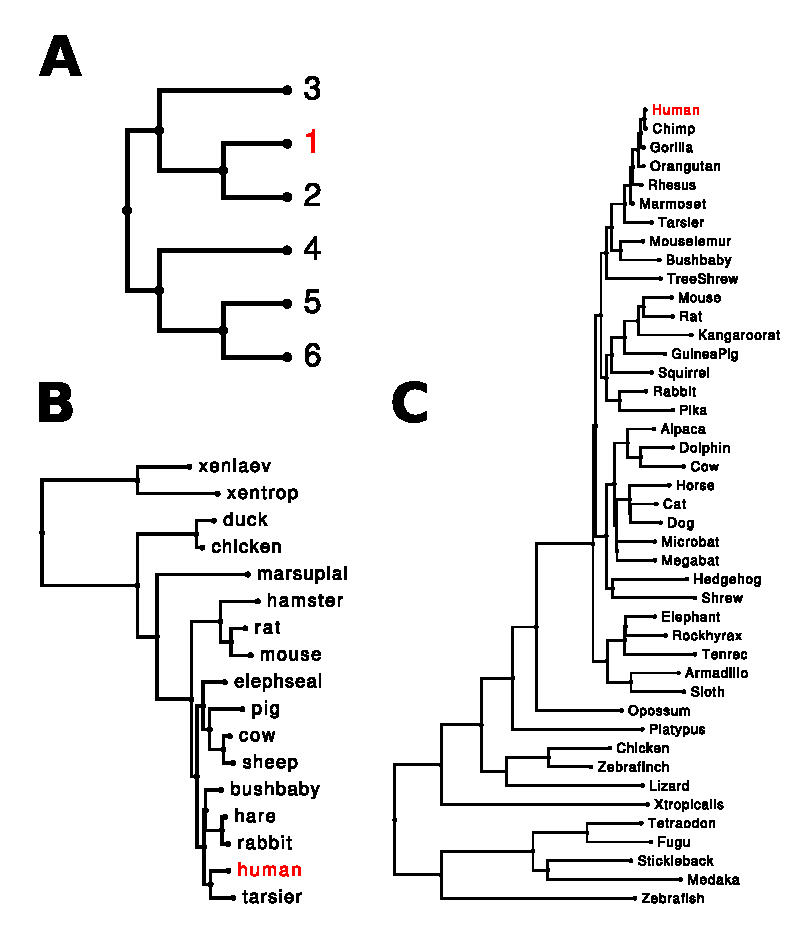
\includegraphics[scale=0.5]{fig1.pdf}
\end{center}
\caption{Phylogenetic trees used for simulation and analysis in this
  article. (a) An artificial tree used in previous simulations
  \citep{Anisimova2001Accuracy,Massingham2005Detecting}. (b) A tree
  estimated from b-globin genes of 17 vertebrates and used in previous
  empirical analyses and simulation studies
  \citep{Anisimova2001Accuracy,Anisimova2002Accuracy}. (c) The
  44-taxon tree used by the ENCODE project
  \citep{2007Identification,Nikolaev2007Early}. The nodes labeled in
  red were used as the reference species (see Methods).}
\label{fig_1}
\end{figure}

The Indelible program \citep{Fletcher2009INDELible} was used to
simulate codon sequences with indels along each phylogenetic tree. The
length of the root sequence was set to 500 codons, $\bm{\kappa}$ (the
ratio of transition to transversion substitutions) was fixed at 4, and
100 replicate alignments were simulated for each set of
conditions. Indel lengths were drawn from a discretized power-law
distribution with an exponential decay parameter of 1.8 and a maximum
value of 40, yielding a mean indel length of 3.33 codons and standard
deviation of 5.51 codons. This power-law model of indel lengths is
well-supported by empirical studies
\citep{Benner1993Empirical,Cartwright2009Problems} and it was decided
after manual inspection of alignments from a range of parameter values
that the chosen model parameters resulted in alignments most closely
resembling those encountered in vertebrate alignments. The ratio of
insertion to deletion events was set to 1, and the rate of indel
formation was scaled from between 0 to 0.2 indel events per
substitution per site.

The distribution of sitewise selective pressures was modeled with a
log-normal distribution derived from a maximum-likelihood fit to a
large dataset of sitewise selective pressures estimated from mammalian
gene trees (log-normal parameters shown in Table 1). This
distribution, with mean w of 0.28 and 6\% of sites having w>1, is
consistent with the structure-based expectation of many protein sites
under purifying selection and few under neutral selection or positive
selection
\citep{Smith1970Natural,Kimura1974SomePrinciples}. Indelible's general
discrete model of sitewise w variation was used to approximate this
distribution by splitting the lognormal probability density into 50
equally-spaced bins between w values of 0 and 3, with the highest bin
containing the probability density for all values w>=3.

Branch lengths for each of the simulation trees were multiplied by a
correction factor before simulation to correct for the difference
between our definition of branch lengths as the number of synonymous
substitutions per synonymous site ($dS$) and Indelible's
interpretation of branch length as the average number of substitutions
per codon ($t$) \citep{Fletcher2010Effect}. They are related
approximately by $t = 3(NdN + SdS) = 3dS(\omg{}N + S)$, where $N$ and
$S$ are the proportion of nonsynonymous and synonymous sites and
$\omg{}$ is the mean $\omg{}$ across all sites. S is approximately 0.3
when $\bm{\kappa}=4$ and the mean $\omg{}$ ratio for our chosen
distribution is 0.277, yielding a $dS$-to-$t$ conversion factor of
1.48 for all simulations performed.

\subsection*{Sequence Alignment and Filtering}

Alignments were inferred using four alignment algorithms chosen for
their widespread use or demonstrated accuracy: ClustalW v1.82
\citep{Thompson1994ClustalW}, MAFFT \citep{Katoh2005MAFFT} and two
variants of PRANK \citep{Loytynoja2005From} based on an amino acid
model (subsequently referred to as \pranka{}) or an empirical codon
model (subsequently referred to as \prankc{}). Unaligned amino acid
sequences were given as input to all alignment programs (except
\prankc{}, which was provided the unaligned DNA sequences) and all
software was run using default parameters with the true phylogenetic
tree given as input where possible.

Alignments were filtered by masking out residues based on the output
of four alignment scoring methods: Gblocks conserved blocks
\citep{Castresana2000Selection}, T-Coffee consistency scores
\citep{Notredame2000TCoffee,Notedame2003Using}, and GUIDANCE alignment
confidence scores \citep{Penn2010Alignment}. Gblocks, which identifies
entire alignment columns as conserved or not conserved, was run using
a relaxed gap allowance parameter in order to avoid removing too much
of the alignment (command-line parameter 'b5=a') and all residues from
any columns not within an identified conserved block were masked with
'N's. GUIDANCE and T-Coffee, which produce individual scores for each
residue, were handled differently. (TODO!!!!). GUIDANCE was run with 30
bootstrap replicates and MAFFT as the bootstrap aligner (except when
\pranka{} or \prankc{} was the original aligner, in which case \pranka{}
was used to align the bootstrap replicates), and T-Coffee was run
using default settings and the 'evaluate\_mode -output=score\_ascii'
command-line parameter to output alignment scores.

Two unrealistic datasets were produced to serve as controls. First,
the true simulated alignment was used in order to evaluate the
sitewise performance without any alignment error. Second, an
additional filtering method was designed to represent an unattainable
best-case scenario for sequence filtering, using knowledge of the true
alignment to assign a score to each residue that summarizes how
correctly is has been placed in the inferred alignment. The approach
taken was to calculate, for each residue, the branch length of the
correct sub-tree (defined as the minimum sub-tree connecting all
sequences to which the current residue is correctly aligned) divided
by the branch length of the aligned sub-tree (defined as the minimum
sub-tree connecting all sequences with non-gap residues at the current
alignment column). This residue-wise score ranges from 0 to 1 and
encapsulates the expectation that correctly-aligned evolutionary
branch length is the main source of information from which the
sitewise inference methods derive their power. Scores from this
method, referred to as the Optimal method, were used to filter
inferred alignments in a manner similar to the T-Coffee and GUIDANCE
scores.

\subsection*{Sitewise Evolutionary Analysis}

Sitewise estimates of selective pressures were calculated using
maximum-likelihood methods implemented in the Phylogenetic Analysis by
Maximum Likelihood (PAML, \citealt{Yang2007PAML}) and Sitewise Likelihood Ratio
(SLR, \citealt{Massingham2005Detecting}) software packages.

The codeml program from PAML implements a number of likelihood ratio
tests (LRTs) for detecting the presence of positive selection in a
gene while allowing the $\omg{}$ ratio to vary among sites
\citep{Yang2000CodonSubstitution}. These models, known as the sites or
random sites models, use a variety of predefined statistical
distributions to account for heterogeneous w ratios among sites. After
the likelihood optimization is performed, Bayesian methods can be used
to estimate the posterior probability of each site being drawn from a
given site class, where a high posterior probability of a site
belonging to a class with $\omg{}>1$ can be considered strong
evidence that a site has evolved under positive selection
\citep{Yang2005Bayes}. We used the two models for which the
recommended Bayes Empirical Bayes method are implemented, M2a and M8.

SLR implements a method specifically designed for sitewise estimates
which has been shown in simulations to perform as well or better than
PAML's sitewise models \citep{Massingham2005Detecting}. SLR models
codon evolution as a continuous-time Markov process where
substitutions at one site are independent of substitutions at all
other sites. Importantly, no assumptions are made regarding the
distribution of $\omg{}$ ratios within the alignment. The value
of $\omg{}$ is considered to be an independent parameter at each
site: after first optimizing shared parameters using the whole
alignment, SLR uses the shared parameters and the data at each
alignment site to calculate a sitewise statistic for non-neutral
evolution. This statistic is based on a likelihood-ratio test where
the null model is neutral evolution ($\omg{}=1$) and the
alternative model is either purifying or positive selection
($\omg{}<1$ or $\omg{}>1$, respectively). The raw statistic
measures the strength of evidence for non-neutral evolution at each
site; following Massingham \citeyearpar{Massingham2005Detecting} we
use a signed version of the SLR statistic (created by negating the
statistic for sites with $\omg{}<1$) as the test statistic for
positive selection.

\subsection*{Measuring Performance}

In order to compare sitewise estimates from different alignments, a
single sequence from each tree was chosen as the reference (red
labels, Figure 1) and all sitewise statistics were mapped from
alignment columns to sequence positions in the reference
sequence. This approach bears some resemblance to the process of
mapping alignment-based evolutionary inferences onto a single member
of the alignment for further analysis and integration with other
genome-referenced data (as is often done, for example, using mammalian
alignments and a human reference). As a result of this reference
sequence based mapping, sites which were deleted in the reference
sequence or inserted in a lineage not ancestral to the reference were
dropped from the analysis.

To evaluate the power and error rates that might be achieved in
real-world data analysis, the recommended cutoff thresholds for PAML’s
Bayesian posterior probabilities and the SLR statistic were used to
identify positively selected sites. A posterior probability threshold
of 0.95 was used for PAML \citep{Yang2005Bayes} and a threshold of 3.84,
the 95\% critical value of the chi-square distribution with 1 degree
of freedom, was used for SLR \citep{Massingham2005Detecting}. Sites were
compared to their true simulated state (e.g. positively-selected or
non-positively selected) in order to identify correct and incorrect
inferences, and from these classifications we calculated the false
positive rate (FPR, defined as the proportion of all sites with true
$\omg{}<1$ falsely identified as positively selected) and true positive rate
(TPR, defined as the proportion of all sites with true $\omg{}>1$ correctly
identified as positively selected).

As the addition of alignment error is expected to affect the power and
error rates differently for each combination of simulation condition
and aligner, we also identified the score thresholds for each dataset
that resulted in an actual FPR of 1\% and calculated the TPR achieved
at this actual error rate (referred to as \tpr{} to distinguish it
from the TPR described above). Although this estimate of
error-controlled power would be impossible to calculate in an
empirical analysis where the error rate is unknown, it is useful in a
simulation context for allowing a controlled comparison of the
performance of sitewise analysis between different
conditions. Specifically, it should be sensitive both to increased
error rates from alignment error and to reduced power from alignment
filtering, in both cases showing a lowered error-controlled power as
the method performs worse.

\section*{Results and Discussion}

\subsection*{Performance of Three Methods for the Sitewise Detection of Positive Selection}

\begin{figure}[h]
\begin{center}
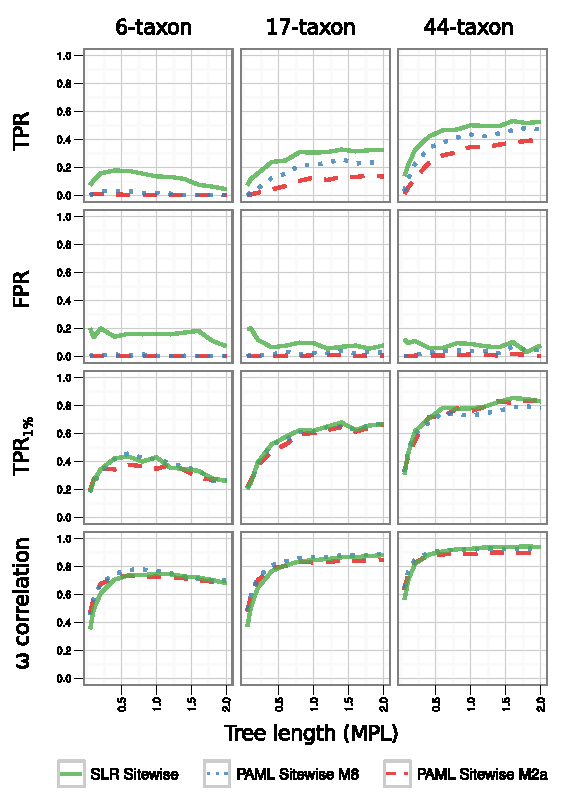
\includegraphics[scale=0.75]{fig2.pdf}
\end{center}
\caption{The behavior of three methods of sitewise inference in the
  absence of indels. One hundred replicate alignments were simulated
  without indels for each tree and divergence level and were analyzed
  with either PAML M2 (red), PAML M8 (blue), or SLR. The performance
  of each method, as measured by four summary statistics, is plotted
  as a function of divergence level. From top to bottom: TPR at the
  recommended cutoff threshold (0.95 for PAML and 2.71 for SLR), FPR
  at the recommended cutoff threshold, TPR at a 1\% FPR threshold, and
  Pearson's correlation coefficient between the true and estimated
  $\omg{}$.}
\label{fig_2}
\end{figure}

We first evaluated the ability of three sitewise methods, PAML M2,
PAML M8 and SLR, to accurately estimate sitewise $\omg{}$ values and to
detect positive selection under a range of tree lengths in the absence
of alignment error. Figure 2 shows the TPR, FPR, \tpr{} and sitewise $\omg{}$
correlation over a range of MPLs for each of the three simulation
trees.

The detection power and ω correlation were weakest at low divergence
levels for all methods and all trees due to the low amount of
evolutionary information, as observed in previous simulations
\citep{Anisimova2002Accuracy}. Also confirming previous results, we
found a positive correlation between tree size and detection power,
with the highest values in the 44-taxon tree. Power generally
increased monotonically with divergence, except for the 6-taxon tree
which saw its maximum performance at moderate divergence levels (MPL
0.5-1.0) and began decreasing at higher values. The downward trend in
the 6-taxon tree was likely due to the impact of saturation of
synonymous sites in the very long branches present in such a sparse
tree at high divergence levels. The two larger trees, with lower
average branch lengths at equivalent divergence levels, showed less
susceptibility to saturation of substitutions along a single
branch. Interestingly, the two larger trees showed no signs of
decreased performance even at a MPL of 2 substitutions per site, which
is greater than any of the divergence levels found in groups of
commonly analyzed vertebrate, insect and fungal species (Table ST1).

Comparing between the three sitewise methods, we found that at the
recommended cutoff threshold (Figure 2, top row) SLR showed the
highest power to detect positive selection in all trees, followed by
PAML M8 and PAML M2. In the smallest tree, the power of the two PAML
methods was virtually zero while SLR reached a maximum of ~18\% TPR at
MPL=0.5. SLR showed a large increase in power in the larger trees
compared to the smallest tree, yielding ~25\% and ~45\% TPR at MPL=0.5
in the 17-taxon and 44-taxon trees, respectively. The two PAML methods
also showed increased power in the larger trees, with PAML M2 ranging
between 50-75\% of SLR’s power and the performance of PAML M8 falling
in between the two other methods.

The TPR measurements represent the power that might be achieved in
real-world analysis using recommended cutoff thresholds, but SLR’s
higher power may reflect merely a shifted balance between power and
accuracy at the recommended cutoff threshold as opposed to an
increased ability to discriminate positive from neutral or purifying
selection. The FPR and error-controlled \tpr{} results showed the
former to be the case. The FPR from SLR was higher than that from
either of the PAML methods for all trees and divergence levels (Figure
2b), suggesting that its higher power was the result of a
less-conservative cutoff rather than significantly improved
statistical performance. This hypothesis was confirmed by evaluating
the TPR at a cutoff threshold for each method that controlled for an
actual FPR of 1\% (\tpr{}, shown in Figure 2c), yielding virtually
identical \tpr{} values for all three methods. The highly similar
error-controlled power levels indicate that the three methods’
sitewise statistics were nearly equally sensitive to positive
selection under these simulation conditions.

The conservative nature of the default thresholds for PAML and SLR
have been previously noted
\citep{Anisimova2002Accuracy,Yang2005Bayes,Massingham2005Detecting}
and the extremely low false positive rates in our simulations
confirmed that all three methods would yield very few false positives
with a realistic distribution of $\omg{}$ values across a range of
tree sizes and divergence levels. For the purposes of our indel
experiments, the observed similarity in error-controlled power levels
indicated that the behavior of PAML M2, PAML M8, and SLR was similar
enough not to warrant separately evaluating all three methods in the
subsequent indel simulation experiments. As the runtime for SLR was
significantly lower than that of either PAML model, all subsequent
results are presented only based on the SLR test.

\subsection*{Effect of Alignment Error on Sitewise Power}

When the indel rate was greater than zero, performance levels varied
significantly for different tree sizes, alignment algorithms, and
evolutionary divergences. Figure 3 shows the same sitewise
measurements as Figure 2 for simulations without indels and with
indels, analyzed using three different aligners and the true
alignment. The indel rate was held constant at 0.1 indel event per
substitution, and the divergence level was varied between 0.2 and 2.0
substitutions per site.

\begin{figure}[t]
\begin{center}
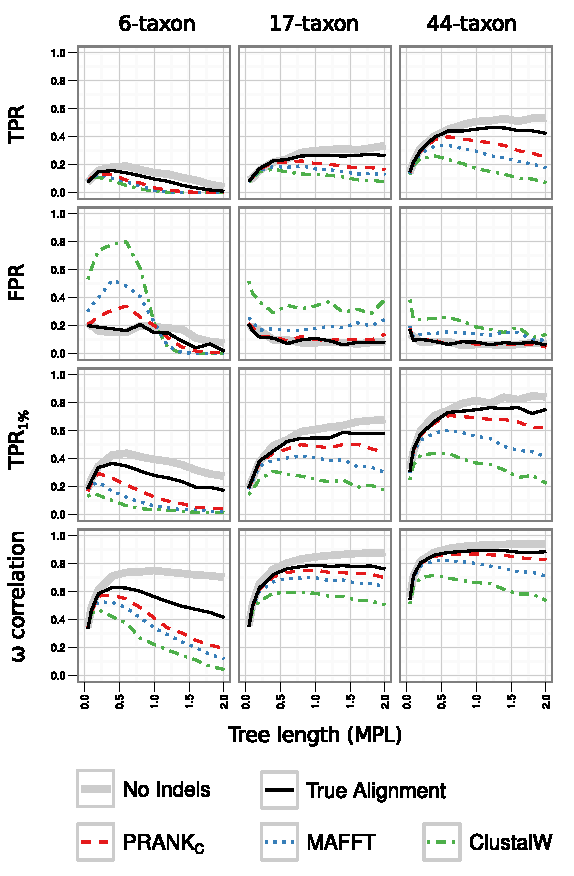
\includegraphics[scale=0.75]{fig3.pdf}
\end{center}
\caption{The behavior of sitewise inference in the presence and absence of indels using three different aligners and the true alignment.}
\label{fig_3}
\end{figure}

Comparing the results without indels to those with indels under the
true alignment (shown as solid black and solid red lines in Figure 3)
we found a slight decrease in power and ω correlation and no
noticeable increase in FPR. The decreased power was expected, since
even in the absence of alignment error, alignment columns containing
gaps harbor less evolutionary information than columns flush with
sequence data. The lack of increased FPR showed that SLR retained its
conservative statistical performance even when analyzing gapped
alignments with indels. Surprisingly, at higher divergences (MPL $>$
1.0) under the six-taxon tree, the FPR with indels was lower than the
FPR without indels. This unexpected result may be attributed to the
large number of alignment columns under such conditions that contain
only a single non-gap sequence, as these columns are never inferred as
positively-selected by SLR due to the complete lack of
information. The two larger trees did not show a similar trend at high
divergence levels, suggesting that the effect was due mainly to the
highly sparse nature of the alignment in the 6-taxon tree. The rest of
our results from the 6-taxon tree at high divergences were similarly
anomalous in this respect; we surmised that the sparseness of the true
alignment combined with the extreme difficulty of accurately aligning
sequences along very long branches made sitewise analysis with indels
very unreliable at high divergences in the smallest tree.

When alignments were inferred using one of the three aligners tested,
the TPR, \tpr{} and $\omg{}$ correlation were all reduced relative to
the true alignment (dashed and dotted red lines, Figure 3A, B, D). The
degree of reduction varied depending on the aligner, simulation
conditions, and performance measurement being analyzed. At low
divergences (e.g. MPL $<$ 0.2), the inferred alignments generally
showed only a small decrease in performance, but the \tpr{} in the
6-taxon tree was a notable exception with large differences down to a
MPL of 0.1. As divergence levels increased, so did the difference
between the performance of the true alignment and the inferred
alignments. The three aligners tested could be consistently and
unambiguously ranked by each of the measured performance
characteristics, with \prankc{} always performing best and ClustalW
performing worst. The same ranking of aligners with respect to
detecting positive selection was found by Fletcher and Yang
\citeyearpar{Fletcher2010Effect}; our results corroborate their
finding and provide evidence that this ranking may be applicable to a
wider array of evolutionary analyses than the branch-site tests
evaluated in their analysis.

When alignments were inferred using one of the three aligners tested,
the TPR, \tpr{} and $\omg{}$ correlation were all reduced relative to
the true alignment (dashed and dotted red lines, Figure 3A, B, D). The
degree of reduction varied depending on the aligner, simulation
conditions, and performance measurement being analyzed. At low
divergences (e.g. MPL < 0.2), the inferred alignments generally showed
only a small decrease in performance, but the \tpr{} in the 6-taxon
tree was a notable exception with large differences down to a MPL of
0.1. As divergence levels increased, so did the difference between the
performance of the true alignment and the inferred alignments. The
three aligners tested could be consistently and unambiguously ranked
by each of the measured performance characteristics, with \prankc{}
always performing best and ClustalW performing worst. The same ranking
of aligners with respect to detecting positive selection was found by
Fletcher and Yang \citeyearpar{Fletcher2010Effect}; our results
corroborate their finding and provide evidence that this ranking may
be applicable to a wider array of evolutionary analyses than the
branch-site tests evaluated in their analysis.

We found that FPR levels under inferred alignments were generally
higher than under the true alignment. This effect was especially
strong in the 6-taxon tree at medium divergence levels (e.g. MPL
0.2-0.6), where ClustalW showed up to a fourfold increase, and \prankc{}
a nearly twofold increase, in FPR over the true alignment. As
previously noted, the 6-taxon tree showed an unexpected and presumably
anomalous FPR pattern at higher divergences, likely due to the highly
sparse true alignment. In the two larger trees, FPRs from inferred
alignments were less elevated compared to the true alignment and
relatively constant across the range of divergences. ClustalW's FPR
ranged between 0.003 to 0.005, while \prankc{}'s FPR was virtually
identical to the true alignment in both the 17-taxon and 44-taxon
trees.

A comparison of the TPR and FPR results between true and inferred
alignments allows the relative impact of false positive and false
negative errors resulting from misalignment to be quantified. A false
positive resulting from over-alignment of non-synonymous codons would
contribute to an elevated FPR, while a false negative resulting from
non-alignment of homologous codons would contribute to a reduced
TPR. The \tpr{} should be sensitive to both false positives and false
negatives since it measures the TPR when controlling for an actual FPR
of 1\%. Analyzing the TPR results in the 6-taxon tree, the three
aligners formed a cluster of lines well below the true alignment
value, indicating similar tendencies among the different aligners to
produce false negatives in the smaller tree. In larger trees the
different aligners showed a wider spread of TPR values, but even
\prankc{} showed a 5-10\% reduction compared to the true alignment at
MPL$=$1.0. These results show that the introduction of false negatives
is a significant and seemingly unavoidable result of alignment error
at medium to high divergence levels (MPL $>$ 0.5), with even the most
powerful aligner producing a marked reduction in TPR compared to the
true alignment. The FPR levels exhibited a very different trend, with
the widest range of values and highest FPRs in the 6-taxon tree and
the smallest range and lowest values in the 44-taxon
tree. Furthermore, the aligner with the lowest FPR, \prankc{}, had FPR
levels almost identical to those of the true alignment in the 17-taxon
and 44-taxon trees. The FPR results suggest that although false
positives resulting from misalignment are unavoidable in a
moderately-diverged 6-taxon tree, the addition of more taxa to the
tree provided enough information for \prankc{} to yield very few false
positives not in the true alignment. Other aligners, however,
maintained a constant elevated FPR in the two larger trees, indicating
a failure to effectively utilize the additional evolutionary
information present in larger trees to avoid introducing false
positive results.

The results shown in Figure 3 allow us to characterize the combined
effects of alignment error at different commonly analyzed levels of
divergence. For example, at a human-mouse divergence level (MPL $=$
0.2) misalignment had little impact on the TPR regardless of what
aligner was used. However, ClustalW yielded a notably higher FPR than
MAFFT or \prankc{}, and the error-controlled \tpr{} was
correspondingly lower for ClustalW in all three trees. Thus, at small
divergences we found that false positives were thus the main source of
error from misalignment, and different aligners had highly variable
tendencies to produce false positive results. At the higher vertebrate
and Drosophila divergence levels (MPL 0.8-1.0) false negatives became
much more prevalent. The TPR for all inferred alignments was virtually
zero in the 6-taxon tree, underscoring the necessity of including many
species in the analysis of highly diverged sequences. In the larger
trees, \prankc{} resulted in very few additional false positives, but
it suffered a 5-10\% reduction in TPR relative to the true alignment
due to false negatives. Meanwhile, ClustalW showed a 50\% TPR
reduction and maintained a strongly elevated FPR. At higher
divergences and in larger trees, false negatives appear to be the most
persistent alignment error, causing a marked reduction in sitewise
power even with the best-performing aligner.

\begin{figure*}[t]
\begin{center}
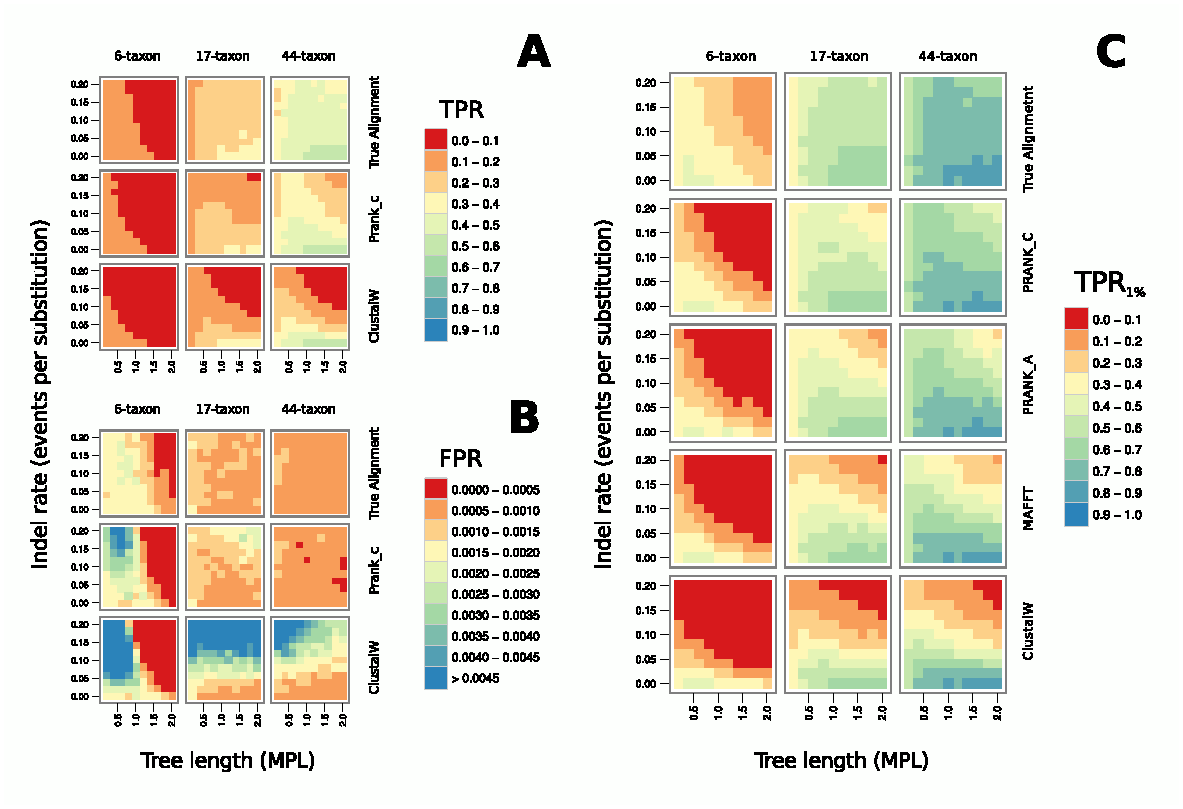
\includegraphics[scale=0.8]{fig4.pdf}
\end{center}
\caption{}
\label{fig_4}
\end{figure*}

\subsection*{Sitewise Power Under a Range of Indel Rates and Divergences}

To explore the effects of alignment error across a wider range of
simulation conditions, we extended the simulations from Figure 3
across a range of indel rates, from 0 to 0.2 indel events per
substitution. Figure 4 shows heatmaps of the TPR and FPR for ClustalW,
\prankc{} and the true alignment (Figure 4A,B) and a heatmap of the
error-controlled \tpr{} for all aligners tested (Figure 4C). The
results from Figure 3, which were simulated with an indel rate of 0.1,
correspond to the middle row of each panel in Figure 4; rows above and
below the middle row represent higher and lower indel rates,
respectively.

The TPR values (Figure 4A) showed a consistent pattern across the
range of indel rates, with power decreasing as either the indel rate
or the divergence level increased. \prankc{} showed a greater ability
than ClustalW to maintain a high TPR at higher indel rates, especially
in the 17-taxon and 44-taxon trees. At lower indel rates, the TPR
performance of both aligners and the true alignment were qualitatively
similar.

\prankc{} and ClustalW both showed a similar tendency towards elevated
FPRs in the 6-taxon tree (Figure 4B), but their behavior diverged
significantly in the 17-taxon and 44-taxon trees. In the 17-taxon
tree, \prankc{} only showed an elevated FPR at very high indel rates
and divergence levels, but the ClustalW FPR consistently increased
with indel rate, quadrupling in value from the lowest to highest indel
rate. Interestingly, for any given indel rate, the ClustalW FPR showed
little variation across the range of divergence levels. This result
was counter-intuitive, as we expected alignment errors to become more
common as divergence increases and the number of observed indel events
grows. Furthermore, \prankc{} behaved according to our expectations,
with a trend towards increased FPRs at higher divergences in the
17-taxon tree and the highest indel rate. The FPR results in the
44-taxon tree confirmed the strange effect of ClustalW’s alignments on
the sitewise FPR: at the highest indel rates, ClustalW showed a
negative correlation between FPR and divergence -- exactly opposite to
the trend we expected.

Finally, the error-controlled \tpr{} results (Figure 4C) provided a
comprehensive map of the effect of alignment error on detecting
sitewise positive selection. The two aligners not shown in the two
other panels, MAFFT and \pranka{}, exhibited \tpr{} values
intermediate to those from ClustalW and \prankc{} across the range of
parameters tested. At indel rates above 0.1, all aligners yielded low
\tpr{} values in the 6-taxon tree. In the larger two trees, excessive
false positives introduced by ClustalW and MAFFT alignments precluded
them from achieving high \tpr{} at high indel rates, while \pranka{}
and \prankc{} showed good \tpr{} levels at all but the highest
divergences and indel rates.

It is worth noting the exceptional ability of PRANK to maintain a low
level of false positive sites even under extremely difficult alignment
conditions. Although \prankc{} showed slightly elevated FPRs at high
indel rates in the 17-taxon tree, FPRs were nearly identical to the
true alignment across all simulated conditions in the 44-taxon
tree. This impressive performance suggests that, given a large enough
number of taxa, PRANK alignments would yield very few erroneous false
positives in scans for positive selection in sequences with divergence
levels well beyond those found in commonly analyzed vertebrate, insect
and fungal clades (Table ST1). Furthermore, these results showed that
false negatives contributed more than false positives to PRANK’s
reduction in sitewise performance --- a novel observation which
provides insight into the nature of PRANK alignments and their
application to sitewise evolutionary analysis.

\subsection*{Effect of Alignment Filtering on Sitewise Error Rates}

\begin{figure*}[t]
\begin{center}
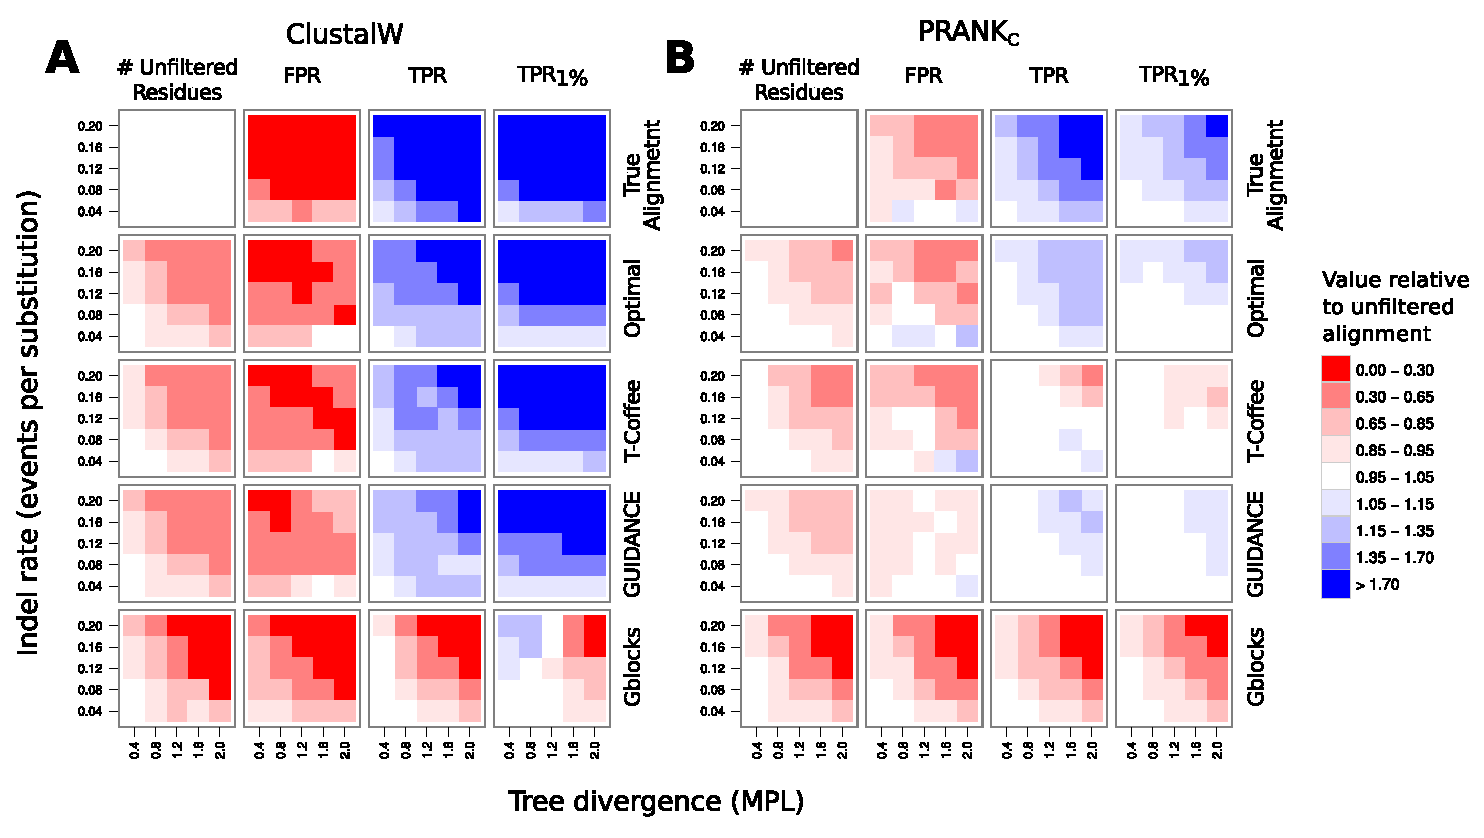
\includegraphics[scale=0.8]{fig5.pdf}
\end{center}
\caption{}
\label{fig_5}
\end{figure*}

Having established that alignment error can lead to reduced sitewise
performance through the introduction of false negatives and false
positives we tested whether a number of alignment filtering methods
could reduce error rates and improve the power of sitewise detection
of positive selection. Using sequences simulated from the 17-taxon
tree and the same range of indel rates and divergence levels as in the
previous experiments, we calculated inferred alignments using ClustalW
and \prankc{} and applied four filtering methods to the alignments
before performing the sitewise analysis. Since we wished to determine
whether alignment filters either improved or worsened the error rate
and power of sitewise analysis, we measured the ratio of each
performance measure to the value obtained in the equivalent unfiltered
dataset. These relative scores are presented in Figure 5.

We first looked at the two controls included in this set of
experiments, the unfiltered true alignment and the inferred alignments
filtered with the optimal filter (Figure 5, top two rows). The true
alignment always showed reduced FPR and increased TPR, and \tpr{}
compared to the inferred alignments, generally with a with greater
magnitude of change compared to the ClustalW alignments than to the
\prankc{} alignments. These relative scores represented the direction
and magnitude of change that might be achieved by an effective
alignment filter. Our hypothesis was that the optimal filtering method
would show the same direction of change in FPR and TPR as the true
alignment. When applied to ClustalW alignments (Figure 5a), the
optimal filter indeed showed a clear pattern of improved sitewise
performance across the majority of simulation conditions, with reduced
FPR and elevated TPR and \tpr{}. At the highest indel rates and
divergence levels, however, little change was observed. This may have
been due to the combination of our filtering limit of 20\% masked
residues and the highly inaccurate nature of ClustalW alignments under
those conditions, as evidenced by the low TPRs and high FPRs in the
previous set of simulations (Figure 4A,B). When applied to \prankc{}
alignments, the optimal filter showed a similar reduction of FPR
levels across the parameter space, but the TPR and \tpr{} results were
mixed. At lower indel rates and divergence levels the TPR and \tpr{}
were reduced, while at higher indel rates and divergences both the TPR
and \tpr{} were slightly increased. The beneficial impact on power
levels under the more difficult alignment conditions sugested that the
optimal filter was able to successfully remove misaligned residues
that were contributing to false negatives in the \prankc{}
alignments. We suspect that the worse performance under easier
alignment conditions was due to the small number of false positives
and false negatives in those \prankc{} alignments, causing any amount
of filtering to result in reduced performance.

When interpreting the results from filtered alignments, we must keep
in mind that alignment filters act through removing alignment residues
or columns, resulting in a certain amount of reduction in the FPR and
TPR purely from the removal of information from the alignment. For
example, a filter that randomly removed a fraction of residues of each
alignment would be expected to produce equal reductions in FPR and TPR
levels. An effective filter that removes false positives may also
yield a reduced TPR, but the FPR reduction would be larger in
magnitude, making the detection of positive selection more powerful at
a given error rate. Thus, a reduced FPR is not necessarily indicative
of good filtering performance, nor is a reduced TPR necessarily
indicative of poor filtering performance. Furthermore, the prevalence
of false negatives resulting from misalignment suggests that alignment
filters may also improve power by removing false negatives, perhaps by
masking out misaligned residues that were preventing positive sites
from being identified. The removal of false negatives would result in
an increased TPR, further complicating the assessment of filtering
results based on FPR or TPR alone. As a result, we preferred the use
of the change in error-controlled \tpr{} when evaluating whether a
filter had successfully improved the sitewise power of a dataset,
since this value is sensitive to changes in both the FPR and TPR.

Using the change in \tpr{} as a measure of filtering performance, we
found T-Coffee and GUIDANCE to be highly effective at improving
ClustalW alignments, with magnitudes of improvement near to those from
the optimal filter. Interestingly, GUIDANCE showed increased
performance at the highest indel and divergence levels, where the
optimal filter had no effect. As with the optimal filter, results were
mixed when applying these two filters to the \prankc{} alignments: at
lower indel rates and divergences both filters resulted in reduced
performance, while T-Coffee achieved modest improvements while
GUIDANCE showed no change under more difficult conditions.

Gblocks behaved very differently from the other filters tested,
resulting in reduced FPR, TPR, and \tpr{} values under nearly all
simulation conditions. Only at high indel rates and low divergence
levels in the ClustalW alignments did Gblocks show an increased \tpr{}
relative to the unfiltered alignments. The poor performance of Gblocks
was likely due to overly-aggressive removal of alignment
columns. Since the program only identifies conserved blocks as opposed
to scoring residues or alignment columns, we could not cap the amount
of masked sequence as was done for the residue-wise filters. Even
though a relaxed setting was used which allowed conserved blocks to
contain gapped regions (see Methods), the dramatically reduced TPR
levels indicate that much of the power to detect positive selection
was eliminated by Gblocks filtering. Dessimoz et
al. \citeyearpar{Dessimoz2010Phylogenetic} found a similar result for
the effect of Gblocks on the accuracy of phylogenetic inference,
suggesting that Gblocks filtering tends to reduce, rather than
increase, the power and accuracy of a number of evolutionary analyses.

Overall, our alignment filtering simulations found that filtering
methods based on GUIDANCE and T-Coffee scores showed a good ability to
remove false positives and false negatives from ClustalW alignments,
with levels of improvement on par with those obtained with the optimal
filter. This was the case across a wide range of divergence levels and
indel rates, suggesting that filtering ClustalW alignments with
T-Coffee or GUIDANCE can usually be expected to result in improved
sitewise performance. Alignment filtering proved less helpful when
applied to \prankc{} alignments, with all filters reducing the
sitewise performance except under the most divergent and indel-rich
conditions. Importantly, alignment filtering only showed improved
performance at divergence levels well above those found in
commonly-analyzed groups of species (e.g., MPL $>$ 1.6). This leads us
to the conclusion that, based on the sample of aligners and filters
tested here, the unfiltered \prankc{} alignments would yield the best
performance for detecting sitewise positive selection when analyzing
protein-coding sequences across a wide range of indel rates and
commonly encountered sequence divergence levels.

\section*{Conclusions}

Sequence alignment is important yet under-studied]

Our simulations showed that alignment error has significant impact on sitewise detection of pos-sel. ClustalW worst, \prankc{} best.

Filtering improves low-quality alignments and high-quality alignments in extreme circumstances, but overall unfiltered \prankc{} is still the best.

Despite high FPRs from ClustalW, false positive rates are still very low... due mainly to conservative cutoff and prevalence of purifying selection in our simulation conditions


(fig.~\ref{sample_fig_2}).



\section*{Acknowledgments}

A.B.H. and P.V. acknowledge ``\'Ecole th\'ematique
g\'enomique environnementale'' for helpful discussions. M. Bormans is
acknowledged for comments on the manuscript. P.V. acknowledges GIS
``G\'enomique marine'' and ``Fondation Total'' and CNRS--ECCO for funding.

\bibliographystyle{mbe3}
\fontsize{9}{10}\selectfont%
\itemsep 0pt

\bibliography{slrsim}
\end{document}
